PaaS clouds host web-accessible (HTTP/S) applications, to which they provide 
high levels of scalability, availability, and resource management. 
PaaS clouds provide scalability by automatically allocating resources 
for applications on the fly (auto scaling), and provide availability through
the execution of multiple instances of the application and/or the PaaS
services they employ for their functionality.
Consequently, viable PaaS technologies as well as
PaaS-enabled applications continue to increase rapidly in number~\cite{paas-growth}.
PaaS clouds provide a high level of abstraction to the application developer that effectively hides
all the infra\-structure-level details such as physical resource allocation (CPU, memory, disk etc), operating
system,
and network configuration. This enables application developers to focus solely on the programming
aspects of their applications, without having to be concerned about deployment issues. But
due to this high level of abstraction, performance monitoring and root cause analysis
is particularly challenging in PaaS clouds. Due to this reason, and the large number of 
PaaS applications available for testing, we design Roots APM to operate within PaaS
clouds.

\begin{figure}
\centering
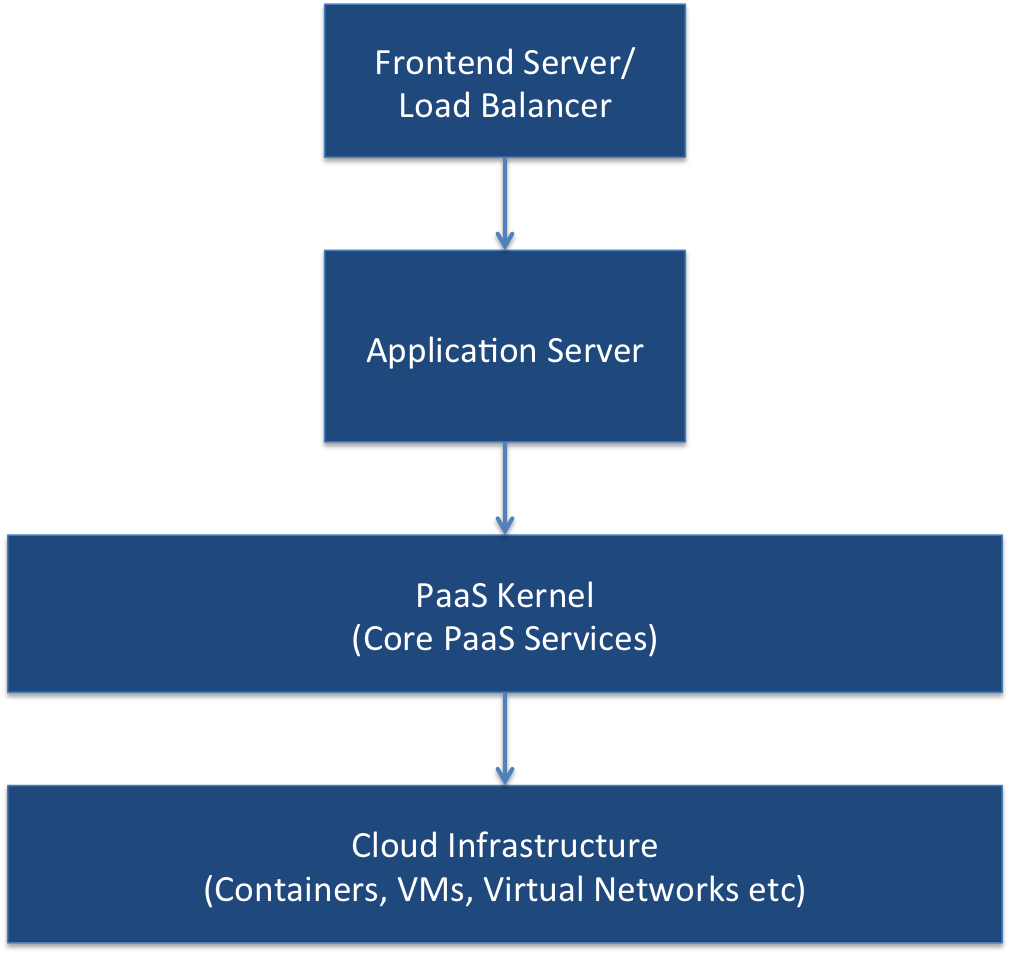
\includegraphics[scale=0.5]{paas_architecture}
\caption{PaaS system organization.}
\label{fig:paas_architecture}
\end{figure}

Figure~\ref{fig:paas_architecture} shows the key layers of a typical PaaS cloud. Arrows indicate
the flow of data and control in response to application requests.

At the lowest level of a PaaS cloud is an infrastructure that consists of the necessary compute, storage
and networking resources. How this infrastructure is set up may vary from a simple cluster of physical 
machines to a comprehensive Infrastructure-as-a-Service (IaaS) solution. In large scale PaaS clouds,
this layer typically consists of many virtual machines and/or containers with the ability to acquire more
resources on the fly.

On top of the infrastructure layer lies the PaaS kernel. This is a collection of managed, scalable
services that high-level application developers can compose into their applications. The provided services
may include database services, caching services, queuing services and much more. Some PaaS clouds
provide a managed set of APIs (an SDK) for the application developer to access these fundamental services. 
In that case all interactions between the applications and the PaaS kernel must take place through
the cloud provider specified APIs (e.g. Google App Engine). 

One level above the PaaS kernel we find the application servers that are used to deploy and run
applications. Application servers provide the necessary integration (linkage) between application code and the
underlying PaaS kernel, while sandboxing application code for secure, multi-tenant operation. On top
of the application servers layer resides the fronted and load balancing layer. This layer is responsible
for receiving all application requests, filtering them and routing them to an appropriate application
server instance for further execution. As the fronted server, it is the entry point for PaaS-deployed
applications for all application clients.

Each of the above layers can span multiple processes, running over multiple physical or virtual
machines. Therefore the execution of a single application request typically involves cooperation
of multiple distributed processes and/or machines. In order to perform comprehensive monitoring
and root cause analysis, we need to be able to monitor each of the above layers along with their
enclosed components. Further we need to be able to trace the flow of data and control
across different layers and components.
